\chapter{Widest Paths}%
\label{chap:08}

\setcounter{section}{1}
\section{Shortest vs.\ Widest Paths}
In the ``classical'' shortest path algorithms discussed so far the length of a
path was given by the \textbf{sum} of the edge weights. In this chapter we
discuss widest path (bottleneck shortest path/ maximum capacity path/ minimax
path) methods.  Here, the length of a path is given by the \textbf{single
  largest} (smallest) edge weight.  \todo{1D example from lecture}

\section{Minimax Paths and Prim's Algorithm}
Recall Disjkstra's Algorithm from a previous lecture. At each iteration we do
the following: take the node $v$ from the list of nodes that have not yet been
visited with the smallest distance from the starting node. Denote by $e = (v,u)$
the edge from $v$ to $u$.  In the ``classical'' Dijkstra algorithm (where we
want to compute the shortest path from the starting vertex to each of the other
nodes) we now do the following: For each edge $e(v,u)$, $u$ in the forward-star
(\ie the set of edges connecting ``outgoing'' nodes) of $v$, update the distance
to the node $u$ according to
\begin{equation*}
  d(u) = \min\{d(u), d(v) + w(e) \}\,,
\end{equation*}
where $w(e)$ is the edge weight of $e$. If we want to compute the minimax path,
we can still use the same idea; however, we instead update $d(u)$ by
\begin{equation*}
  d(u) = \min\{d(u), \max\{ d(v), w(e) \}\}\,,
\end{equation*}
since we are only interested in the single most expensive edge on the way from
the starting node to $u$. This change essentially leads to a related algorithm,
called (eager) Prim's algorithm. Instead of finding the shortest path we now
build a spanning tree, \ie a minimal tree that contains every node of the
graph. We see that the shortest path problem and the minimax problem are in
essence the same problem only with different definition of what we mean by the
distance between two nodes. In other words: both a shortest path problems with a
different notion of what it means to be short. Algebraic graph theory, which is
discussed in the next chapter, provides a unified framework to better understand
this relationship.

\section{All-Pairs Minimax Paths and the Minimum Spanning Tree}
A minimum spanning tree (MST) is a subgraph with the shape of a tree (\ie it
contains no loops) that is spanning (\ie each node can be reached from any other
in the subgraph) whose sum of edge weights is minimal. Every edge not in the MST
is at least as large/ heavy/ costly as all other edges in the loop induced by
adding that edge to a MST (``cycle property''), see Figure~\ref{fig:mst}.
\begin{figure}[htpb]
  \centering 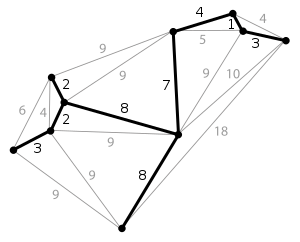
\includegraphics[width=0.6\textwidth]{Figures/MST}
  \caption{A minimum spanning tree.}%
  \label{fig:mst}
\end{figure}

It turns out that the path from some node $u$ to some other node $v$ in the MST
of an undirected graph is a minimax path between $u$ and $v$ in that graph. The
converse is not true in general: the union of the minimax paths between all
nodes is not necessarily a tree and hence in particular it need not be the MST.

Further, in an undirected graph with non-negative edge weights, the minimax
distance between pairs of vertices defines an \textbf{ultrametric}.

\begin{definition*}
  An ultrametric $d_{uv}$ is a metric with the following additional property
  \begin{equation*}
    d_{uv} \le \max\{ d_{uw}, d_{wv}\}\,,
  \end{equation*}
  the so called \emph{strong triangle inequality} (or ultrametric inequality).
\end{definition*}
Note that the ultrametric inequality implies that there exists a permutation
$(i,j,k)$ of three vertices $(u,v,w)$ such that
\begin{equation*}
  d_{ij} \le d_{ik} = d_{kj}\,.
\end{equation*}
This, in turn, implies that a set of points in an ultrametric space can always
be represented as leaves in a binary rooted tree that all have the same distance
from the root (a so called \emph{ultrametric tree}). Consider again the MST from
Figure~\ref{fig:mst}. We can build the corresponding ultrametric tree as
follows. Start with the nodes that have the smallest distance, draw them as
leaves of a tree and connect them to the same parent that is located at the
``height'' that corresponds to their distance (see Figure below; we start with
the two nodes on the top right that are connected by an edge with weight
one). Then we take the node that is next closest and connect the subtree from
the previous step to this node (in the Figure~\ref{fig:ultramteric:tree}, now
all vertices within the green ellipse are processed). We then repeat this
process until no more nodes are left. The ultrametric distance between two nodes
is then given by the height of their least common ancestor in the ultrametric
tree. Note that there exist data structures such that finding the least common
ancestor of two nodes is an $\mathcal{O}(1)$ operation.

\begin{figure}[htpb]
  \centering
  \begin{subfigure}[c]{0.4\textwidth}
    \begin{tikzpicture}
      \node[anchor=south west,inner sep=0] at (0,0)
      {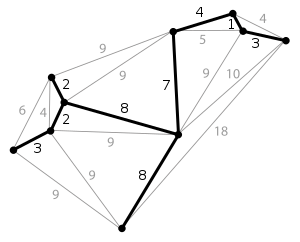
\includegraphics[width=\textwidth]{Figures/MST}};

      \draw[red, rotate around={-60:(5.15,4.7)}] (5.15,4.7) ellipse (0.4cm and
      0.2cm); \draw[green, rotate around={-120:(5.6,4.5)}] (5.6,4.5) ellipse
      (0.5cm and 1cm); \draw[blue, rotate around={0:(5,4.55)}] (5,4.55) ellipse
      (1.5cm and 0.5cm); \draw[cyan, rotate around={0:(4.5,3.7)}] (4.5,3.7)
      ellipse (2cm and 1.6cm); \draw[magenta, rotate around={0:(0,0)}] (1.2,3)
      ellipse (0.3cm and 0.8cm); \draw[olive, rotate around={-40:(0.9,2.9)}]
      (0.9,2.8) ellipse (0.7cm and 1.2cm); \draw[violet, rotate
      around={-50:(3,2.9)}] (3.1,2.9) ellipse (2.1cm and 4cm);
    \end{tikzpicture}
  \end{subfigure}
  \begin{subfigure}[c]{0.4\textwidth}
    \includegraphics[width=\textwidth]{Figures/ultrametric_tree.tikz}
  \end{subfigure}
  \caption{Minimum spanning tree and corresponding ultrametric tree. The
    ultrametric tree is built by repeatedly finding the nodes that have the
    smallest distance to the nodes already processed (indicated by the
    ellipses).}%
  \label{fig:ultramteric:tree}
\end{figure}

\section{Seeded Watershed Segmentation}
The watershed algorithm can be used to segment an image. We begin with a version
of the algorithm where the user has to provide seeds for, \eg foreground and
background classes. Consider the example image in Figure~\ref{fig:watershed}
where we want to partition the image into the two given classes. On the left we
have the original image which has already been transformed into a graph where
the edge weights might come from a neural network or some other means. Starting
from the artificial meta node we compute the minimum spanning tree using Prim's
algorithm. The result is shown on the right.

\begin{figure}[htpb]
  \begin{subfigure}[t]{0.5\textwidth}
    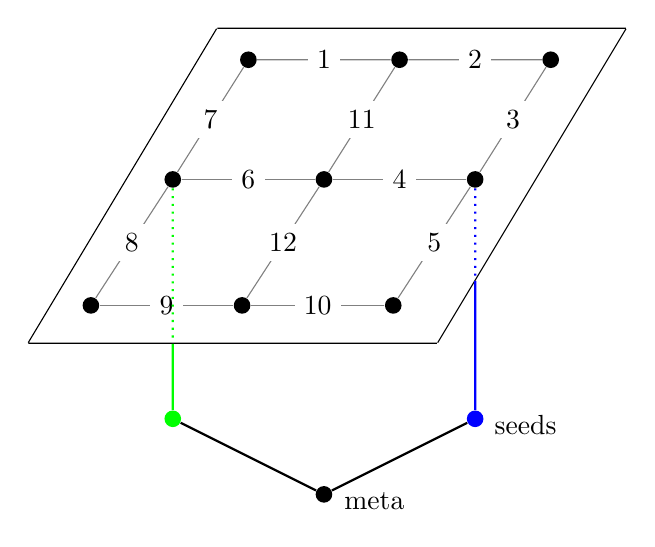
\begin{tikzpicture}[scale=0.8]
      \node[inner sep=0pt,minimum size=0pt] (B1) at (0,0) {};%
      \node[inner sep=0pt,minimum size=0pt] (B2) at (6.5,0) {};%
      \node[inner sep=0pt,minimum size=0pt] (B3) at (9.5,5) {};%
      \node[inner sep=0pt,minimum size=0pt] (B4) at (3,5) {};%

      \node[circle,fill,inner sep=0pt, minimum size=6pt] (P1) at (3.5,4.5) {};%
      \node[circle,fill,inner sep=0pt, minimum size=6pt] (P2) at (5.9,4.5) {};%
      \node[circle,fill,inner sep=0pt, minimum size=6pt] (P3) at (8.3,4.5) {};%

      \node[circle,fill,inner sep=0pt, minimum size=6pt] (P4) at (2.3,2.6) {};%
      \node[circle,fill,inner sep=0pt, minimum size=6pt] (P5) at (4.7,2.6) {};%
      \node[circle,fill,inner sep=0pt, minimum size=6pt] (P6) at (7.1,2.6) {};%

      \node[circle,fill,inner sep=0pt, minimum size=6pt] (P7) at (1,0.6) {};%
      \node[circle,fill,inner sep=0pt, minimum size=6pt] (P8) at (3.4,0.6) {};%
      \node[circle,fill,inner sep=0pt, minimum size=6pt] (P9) at (5.8,0.6) {};%

      \node[circle,fill=green,inner sep=0pt, minimum size=6pt] (GS) at
      (2.3,-1.2) {};%
      \node[circle,fill=blue,inner sep=0pt, minimum size=6pt] (BS) at (7.1,-1.2)
      {};%

      \node[circle,inner sep=0pt, minimum size=0pt] (GSH) at (2.3,0) {};%
      \node[circle,inner sep=0pt, minimum size=0pt] (BSH) at (7.1,1) {};%

      \node[circle,inner sep=0pt, minimum size=6pt,fill] (M) at (4.7,-2.4) {};%
      \node (MT) at (5.5,-2.5) {meta};%
      \node (ST) at (7.9,-1.3) {seeds};%
    
      \draw[-] (B1) -- (B2) -- (B3) -- (B4) -- (B1);%

      \draw[draw=gray] (P1) -- (P2) node[midway,fill=white] {$1$};%
      \draw[draw=gray] (P2) -- (P3) node[midway,fill=white] {$2$};%
      \draw[draw=gray] (P4) -- (P5) node[midway,fill=white] {$6$};%
      \draw[draw=gray] (P5) -- (P6) node[midway,fill=white] {$4$};%
      \draw[draw=gray] (P7) -- (P8) node[midway,fill=white] {$9$};%
      \draw[draw=gray] (P8) -- (P9) node[midway,fill=white] {$10$};%
      \draw[draw=gray] (P1) -- (P4) node[midway,fill=white] {$7$};%
      \draw[draw=gray] (P2) -- (P5) node[midway,fill=white] {$11$};%
      \draw[draw=gray] (P3) -- (P6) node[midway,fill=white] {$3$};%
      \draw[draw=gray] (P4) -- (P7) node[midway,fill=white] {$8$};%
      \draw[draw=gray] (P5) -- (P8) node[midway,fill=white] {$12$};%
      \draw[draw=gray] (P6) -- (P9) node[midway,fill=white] {$5$};%

      \draw[green,dotted,thick] (P4) -- (GSH);%
      \draw[green,thick] (GSH) -- (GS);%

      \draw[blue,dotted,thick] (P6) -- (BSH);%
      \draw[blue,thick] (BSH) -- (BS);%

      \draw[thick] (GS) -- (M) -- (BS);%
    \end{tikzpicture}
    \caption{Original graph}
  \end{subfigure}%
  \begin{subfigure}[t]{0.5\textwidth}
    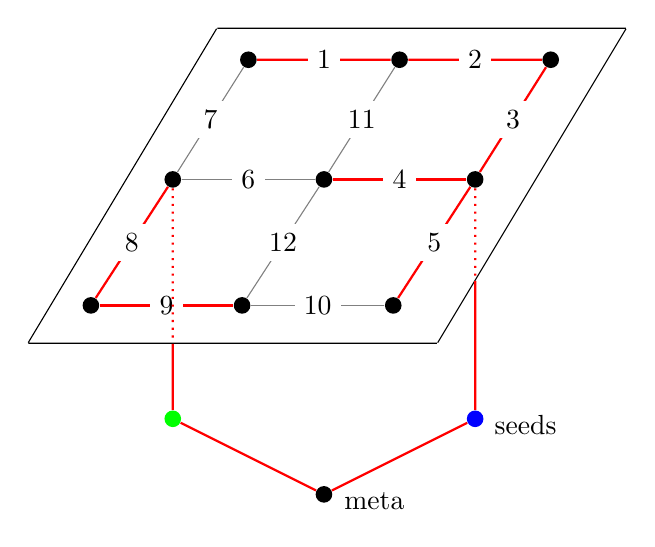
\begin{tikzpicture}[scale=0.8]
      \node[inner sep=0pt,minimum size=0pt] (B1) at (0,0) {};%
      \node[inner sep=0pt,minimum size=0pt] (B2) at (6.5,0) {};%
      \node[inner sep=0pt,minimum size=0pt] (B3) at (9.5,5) {};%
      \node[inner sep=0pt,minimum size=0pt] (B4) at (3,5) {};%

      \node[circle,fill,inner sep=0pt, minimum size=6pt] (P1) at (3.5,4.5) {};%
      \node[circle,fill,inner sep=0pt, minimum size=6pt] (P2) at (5.9,4.5) {};%
      \node[circle,fill,inner sep=0pt, minimum size=6pt] (P3) at (8.3,4.5) {};%

      \node[circle,fill,inner sep=0pt, minimum size=6pt] (P4) at (2.3,2.6) {};%
      \node[circle,fill,inner sep=0pt, minimum size=6pt] (P5) at (4.7,2.6) {};%
      \node[circle,fill,inner sep=0pt, minimum size=6pt] (P6) at (7.1,2.6) {};%

      \node[circle,fill,inner sep=0pt, minimum size=6pt] (P7) at (1,0.6) {};%
      \node[circle,fill,inner sep=0pt, minimum size=6pt] (P8) at (3.4,0.6) {};%
      \node[circle,fill,inner sep=0pt, minimum size=6pt] (P9) at (5.8,0.6) {};%

      \node[circle,fill=green,inner sep=0pt, minimum size=6pt] (GS) at
      (2.3,-1.2) {};%
      \node[circle,fill=blue,inner sep=0pt, minimum size=6pt] (BS) at (7.1,-1.2)
      {};%

      \node[circle,inner sep=0pt, minimum size=0pt] (GSH) at (2.3,0) {};%
      \node[circle,inner sep=0pt, minimum size=0pt] (BSH) at (7.1,1) {};%

      \node[circle,inner sep=0pt, minimum size=6pt,fill] (M) at (4.7,-2.4) {};%
      \node (MT) at (5.5,-2.5) {meta};%
      \node (ST) at (7.9,-1.3) {seeds};%
    
      \draw[-] (B1) -- (B2) -- (B3) -- (B4) -- (B1);%

      \draw[draw=red,thick] (P1) -- (P2) node[midway,fill=white] {$1$};%
      \draw[draw=red,thick] (P2) -- (P3) node[midway,fill=white] {$2$};%
      \draw[draw=gray] (P4) -- (P5) node[midway,fill=white] {$6$};%
      \draw[draw=red,thick] (P5) -- (P6) node[midway,fill=white] {$4$};%
      \draw[draw=red,thick] (P7) -- (P8) node[midway,fill=white] {$9$};%
      \draw[draw=gray] (P8) -- (P9) node[midway,fill=white] {$10$};%
      \draw[draw=gray] (P1) -- (P4) node[midway,fill=white] {$7$};%
      \draw[draw=gray] (P2) -- (P5) node[midway,fill=white] {$11$};%
      \draw[draw=red,thick] (P3) -- (P6) node[midway,fill=white] {$3$};%
      \draw[draw=red,thick] (P4) -- (P7) node[midway,fill=white] {$8$};%
      \draw[draw=gray] (P5) -- (P8) node[midway,fill=white] {$12$};%
      \draw[draw=red,thick] (P6) -- (P9) node[midway,fill=white] {$5$};%

      \draw[red,dotted,thick] (P4) -- (GSH);%
      \draw[red,thick] (GSH) -- (GS);%

      \draw[red,dotted,thick] (P6) -- (BSH);%
      \draw[red,thick] (BSH) -- (BS);%

      \draw[thick,red] (GS) -- (M) -- (BS);%
    \end{tikzpicture}
    \caption{Graph partitioned into two parts using Prim's algorithm starting
      from the meta node}
  \end{subfigure}
  \caption{Seeded watershed algorithm applied to a simple $3 \times 3$ image.}%
  \label{fig:watershed}
\end{figure}

This clearly induces a ``cut'' through the image an we can now assign the upper
right pixels to the blue class and the lower left pixels to the green class. One
can also use the same idea without providing seeds manually but instead choosing
them automatically. In this algorithm which is then simply called
\emph{watershed segmentation}, the local minima of the image are used as
seeds. This can be used in practice to find so called ``superpixels'' to
coarse-grain a computation. These superpixels should lie within one instance in
the image, but they might not fill the entire image; in other words we coarsened
the image but still kept the segments separate. On the graph corresponding to
these superpixels we can then perform seeded watershed algorithm. Also other
variants of watershed are possible where the seeds are found, for example, by a
deep learning method.

We have now discussed two different approaches to perform seeded segmentation:
one using shortest paths and one using minimax paths (watershed) and they can
behave very differently. In the first variant, \ie when using the sum of edge
weights as the cost of a path, the costs obviously accumulate over distance and
thus the proximity of pixels to seed very much matters (\eg very long thin
segments might not be classified as one segment). Thus, a single seed will not
take us very far. However, a segment with an incomplete boundary will not easily
``bleed'' through this boundary which often happens in seeded watershed
segmentation. When using the maximum of edge weights, the cost of a path depends
on the single weakest edge and thus, a single seed can give very large segments.

%%% Local Variables:
%%% mode: latex
%%% TeX-master: "../main"
%%% End:
